\chapter{الترموديناميك الكهروكيميائي للخلايا}\label{ch:b2:cell-thermodynamics}

تحمل حافلة تعمل بخلايا وقود الهيدروجين مكدسًا من بضع مئات من الخلايا الرقيقة. في
كل منها يتحد الهيدروجين وأكسجين الهواء ماءً دون لهب، وتخرج
الطاقة تيارًا كهربائيًا. ويحكم مكدسًا كهذا عددان، يأتي
كلاهما مباشرة من جداول طاقات جيبس: لا تعطي أي خلية أكثر من
\qty{1.23}{V}، ولا تحوّل أي خلية وقود، مهما كملت، كل طاقة
هيدروجينها إلى شغل كهربائي. يربط هذا الفصل جهد الخلية
\omterm{def:b2:reaction-free-energy:gibbs-energy}{بطاقة جيبس} لتفاعلها، ويستنتج معادلة نرنست المستعملة منذ
مجلد السنة الأولى، ويقرأ إنتروبيات التفاعل وأنتالبياته على مقياس
فولط وعلى محرار.

\begin{recall}
مجلد السنة الأولى: الخلايا، وأنصاف الخلايا، والمصعد والمهبط، والجسر الملحي، وجهد
الخلية، وجهد القطب، والجهد المعياري وقطب الهيدروجين
المعياري، ومعادلة نرنست (المقبولة هناك دون برهان)، وثوابت التوازن انطلاقًا من
الجهود. \Cref{ch:b2:reaction-free-energy}: $\Delta_r G$ و$\Delta_r G^\circ$
و$\Delta_r G = \Delta_r G^\circ + RT\ln Q$؛ ومحك التطور.
\Cref{ch:b2:chemical-potential}: النشاطيات. والمجلد المدرسي: التحليل الكهربائي.
\end{recall}

\begin{omfigure}
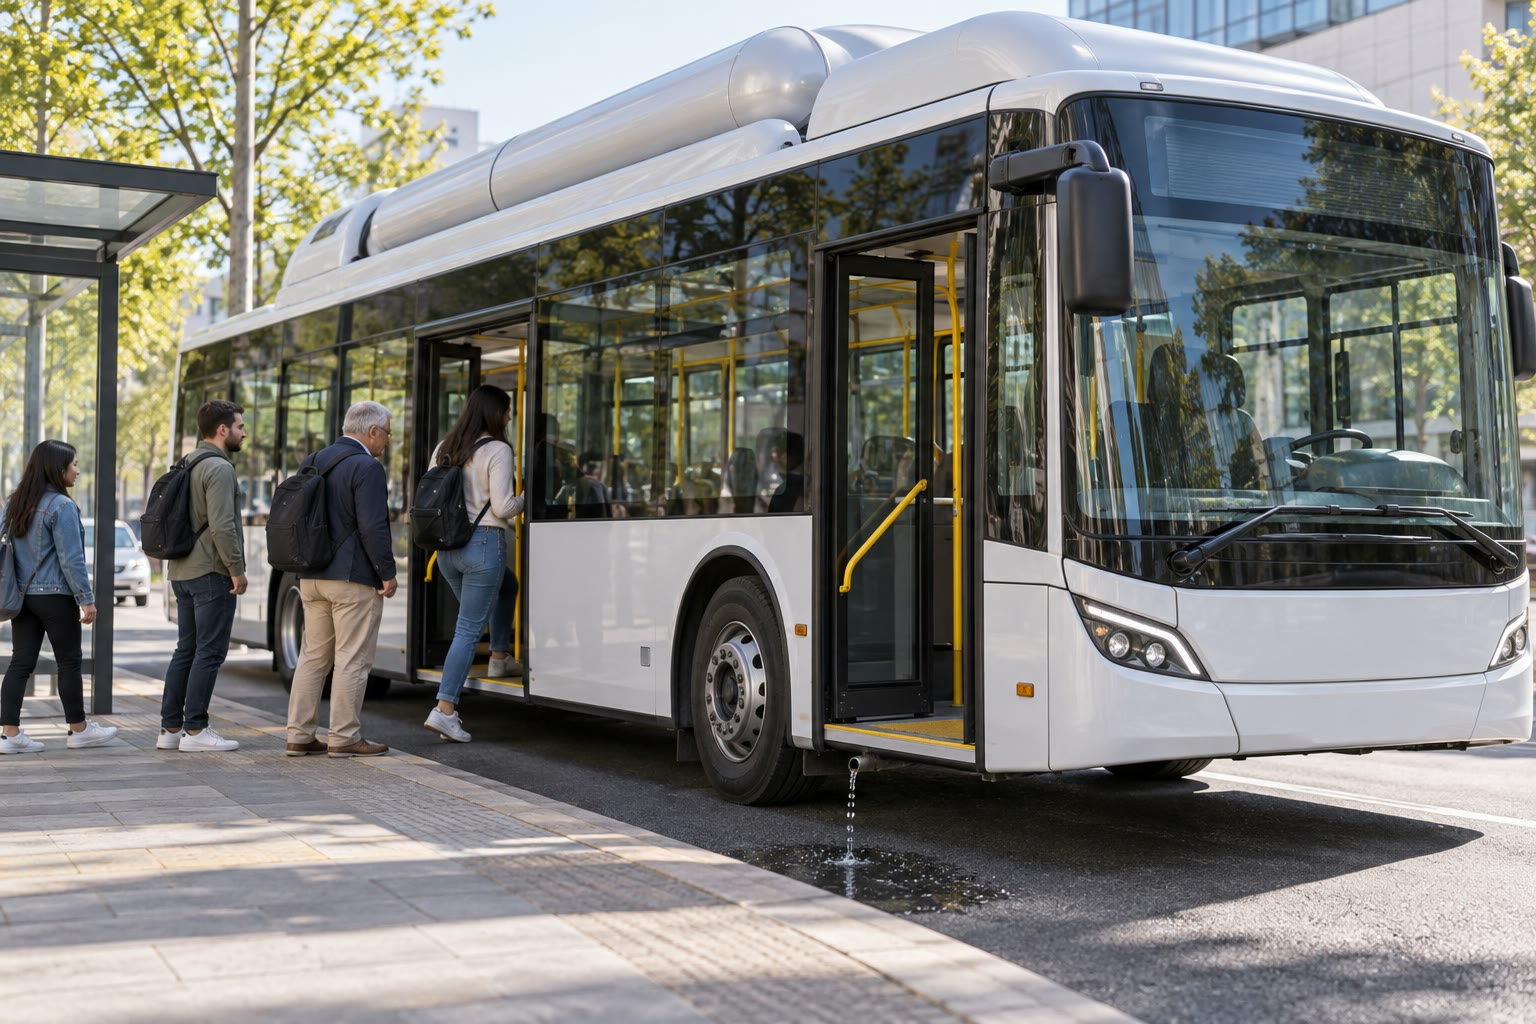
\includegraphics[width=0.62\linewidth]{images/book3/ai/b2-09-fuel-cell-bus.jpg}

{\small حافلة تعمل بخلايا وقود الهيدروجين في محطة: خزانات الهيدروجين تحت
الغطاء على السقف، والعادم الوحيد ماء يقطر تحت الحافلة.}
\end{omfigure}

\section{الشغل الكهربائي وثابت فاراداي}

\begin{definition}[ثابت فاراداي]\label{def:b2:cell-thermodynamics:faraday}
\emph{ثابت فاراداي}\index{ثابت فاراداي} هو الشحنة الكهربائية
لمول واحد من الشحنات الأولية، $F = N_A e = \qty{96485.33}{C/mol}$.
% ledger: const:F
\end{definition}

\begin{proposition}[الشحنة المارة]\label{prop:b2:cell-thermodynamics:charge}
إذا تقدم تفاعل خلية، مكتوبًا مع $n$ إلكترونًا متبادلًا، بمقدار
$\Delta\xi$، فإن الشحنة التي تجري في الدارة الخارجية هي $Q =
nF\,\Delta\xi$.
\end{proposition}

\begin{proof}
التقدم $\Delta\xi$ ينقل $n\,\Delta\xi$ مولًا من الإلكترونات من
المصعد إلى المهبط عبر السلك، شحنة كل منها $e$ بالقيمة المطلقة:
$Q = n\,\Delta\xi\,N_A e$.
\end{proof}

حين تُدفع شحنة $Q$ عبر دارة بجهد $U$، يكون الشغل الذي
تستقبله الدارة $QU$. ومن منظور الخلية، التي تعطي هذا الشغل،
يكون الشغل الكهربائي الذي تستقبله $\delta W_{\text{كهربائي}} = -U\,\delta Q = -nFU\,
d\xi$.

\begin{omfigure}
\begin{tikzpicture}[font=\small, >={Stealth}]
  \draw[thick, rounded corners, fill=omDef!8] (0,0) rectangle (3.2,2.2);
  \node[align=center] at (1.6,1.1) {\shortstack{\foreignlanguage{arabic}{خلية}\\\foreignlanguage{arabic}{(النظام)}\\\foreignlanguage{arabic}{التفاعل $d\xi$}}};
  \draw[->, thick, omThm] (3.2,1.6) -- (5.6,1.6) node[right, align=left] {\foreignlanguage{arabic}{$\delta W_{\text{كهربائي}}$ معطى}\\ $= nFU\,d\xi$};
  \draw[->, thick, omDef] (5.6,0.6) -- (3.2,0.6) node[pos=0, right, align=left] {\shortstack{\foreignlanguage{arabic}{$\delta Q_{\text{حرارة}}$ مستقبَلة}\\\foreignlanguage{arabic}{(إشارتها كيفما كانت)}}};
  \draw[<->, thick] (1.6,2.2) -- (1.6,3.0) node[above] {\foreignlanguage{arabic}{الوسط المحيط عند $T$، $p$}};
\end{tikzpicture}

{\small الخلية نظامًا ترموديناميكيًا عند درجة حرارة وضغط ثابتين:
تتبادل الحرارة مع وسطها المحيط وتعطي شغلًا كهربائيًا عبر
الدارة الخارجية. ومع اصطلاح إشارة المبدأ الأول (الشغل والحرارة
المستقبَلان موجبان)، $\delta W_{\text{كهربائي}} = -nFU\,d\xi$.}
\end{omfigure}

\section{طاقة جيبس لتفاعل الخلية}

\begin{theorem}[الشغل الكهربائي وطاقة جيبس]\label{thm:b2:cell-thermodynamics:delta-g-nfe}
الخلية العاملة عند $T$ و$p$ ثابتين تعطي شغلًا كهربائيًا لا يزيد على
تناقص \omterm{def:b2:reaction-free-energy:gibbs-energy}{طاقة جيبس} لها: فمن أجل تقدم $d\xi$،
$nFU\,d\xi \leq -\Delta_r G\,d\xi$. وحين تعمل عكوسيًا (بتيار
متناهي الصغر)، تتحقق المساواة، ويكون جهد الخلية هو
القوة المحركة الكهربائية
\[
  \Delta_r G = -nFE .
\]
\end{theorem}

\begin{proof}
المبدأ الأول عند ضغط ثابت، مع فصل شغل الضغط:
$dH = \delta Q + \delta W_{\text{كهربائي}}$. والمبدأ الثاني: $dS \geq \delta Q/T$. وعند
$T$ و$p$ ثابتين، $dG = dH - T\,dS \leq \delta W_{\text{كهربائي}} = -nFU\,d\xi$.
ومع $dG = \Delta_r G\,d\xi$، $\Delta_r G\,d\xi \leq -nFU\,d\xi$، أي
$nFU\,d\xi \leq -\Delta_r G\,d\xi$. وفي تحوّل عكوس تصير متراجحة
المبدأ الثاني مساواة، والجهد المقيس عندئذ، دون
تيار، هو $E$: $\Delta_r G = -nFE$.
\end{proof}

لا تستطيع الخلية إذن أن تعمل في الاتجاه المباشر ($d\xi > 0$، معطيةً شغلًا) إلا إذا كان $\Delta_r G <
0$، أي $E > 0$ والقطبان مختاران بحيث يجري التفاعل المكتوب
من المصعد إلى المهبط. أما الخلية الحقيقية، التي يمر فيها تيار، فتعطي
شغلًا أقل من $-\Delta_r G$: ويتبدد الفرق حرارةً في
مقاومتها وعند قطبيها (\cref{ch:b2:current-potential-curves}).

\begin{example}[خلية دانييل]\label{ex:b2:cell-thermodynamics:daniell}
من أجل \ce{Zn + Cu^2+ -> Zn^2+ + Cu}، $\Delta_r G^\circ = \Delta_f G^\circ(\ce{Zn^2+}) -
\Delta_f G^\circ(\ce{Cu^2+}) = -147.06 - 65.49 = \qty{-212.55}{kJ/mol}$، و$n = 2$:
$E^\circ = 212\,550/(2 \times 96\,485) = \qty{1.10}{V}$، وهو الجهد المقيس على
خلية دانييل في الشروط القياسية.
% ledger: dfg:Zn2+_ao, dfg:Cu2+_ao, const:F, emf:Daniell
\end{example}

\section{معادلة نرنست والجهود المعيارية}

قبل مجلد السنة الأولى معادلة نرنست دون برهان؛ وهي الآن تنتج من
$\Delta_r G = \Delta_r G^\circ + RT\ln Q$.

\begin{theorem}[معادلة نرنست، مبرهنةً]\label{thm:b2:cell-thermodynamics:nernst-derived}
من أجل نصف التفاعل $\alpha\,\mathrm{Ox} + n\,\mathrm e^- \rightleftharpoons
\beta\,\mathrm{Red}$، يكون جهد القطب عند درجة الحرارة $T$
\[
  E = E^\circ + \frac{RT}{nF}\ln\frac{a_{\mathrm{Ox}}^{\alpha}}{a_{\mathrm{Red}}^{\beta}} ,
\]
حيث تشمل النشاطيات نشاطيات كل الأنواع الكيميائية الأخرى في
نصف التفاعل (\ce{H+}، ما عدا الماء)، مرفوعة إلى أُسّسها الستوكيومترية.
\end{theorem}

\begin{proof}
جهد القطب هو جهد الخلية المكوّنة من قطب الهيدروجين المعياري
(مصعدًا) ومن ذلك القطب (مهبطًا). وتفاعلها
\[
  \alpha\,\mathrm{Ox} + \tfrac n2\,\ce{H2} \longrightarrow \beta\,\mathrm{Red} + n\,\ce{H+} ,
\]
وخارج تفاعله، مع $a_{\ce{H+}} = 1$ و$p_{\ce{H2}} = p^\circ$ عند
قطب الهيدروجين المعياري، يؤول إلى $a_{\mathrm{Red}}^\beta/
a_{\mathrm{Ox}}^\alpha$. ومن \cref{thm:b2:cell-thermodynamics:delta-g-nfe}،
$E = -\Delta_r G/(nF) = -\Delta_r G^\circ/(nF) - (RT/nF)\ln Q$؛ ومع $E^\circ =
-\Delta_r G^\circ/(nF)$ نحصل على الصيغة. وعند \qty{298.15}{K}، $RT\ln 10/F =
\qty{0.0592}{V}$.
\end{proof}

\begin{proposition}[الجهود المعيارية من طاقات جيبس]\label{prop:b2:cell-thermodynamics:standard-potential}
مع الاصطلاحين $\Delta_f G^\circ(\ce{H+}, \text{aq}) = 0$ 
و$\Delta_f G^\circ(\ce{H2}, \text{g}) = 0$، يكون الجهد المعياري لمزدوجة
$E^\circ = -\Delta_r G^\circ/(nF)$، حيث $\Delta_r G^\circ$ \omterm{def:b2:reaction-free-energy:reaction-gibbs}{طاقة جيبس القياسية}
لنصف التفاعل مكتوبًا اختزالًا، مع عدّ الإلكترونات ذات \omterm{def:b2:reaction-free-energy:gibbs-energy}{طاقة جيبس}
معدومة.
\end{proposition}

\begin{proof}
في التفاعل مقابل قطب الهيدروجين، لا يساهم $\tfrac n2\,\ce{H2}$ 
و$n\,\ce{H+}$ بشيء في $\Delta_r G^\circ$ وفق هذين الاصطلاحين: \omterm{def:b2:reaction-free-energy:reaction-gibbs}{فطاقة جيبس
القياسية لتفاعل} الخلية هي طاقة نصف التفاعل وحده.
\end{proof}

\begin{method}[جهد معياري من الجداول]\label{met:b2:cell-thermodynamics:e-from-gibbs}
\begin{enumerate}
  \item اكتب نصف التفاعل اختزالًا، موزونًا بأيونات \ce{H+} 
        و\ce{H2O}، مع $n$ إلكترونًا.
  \item احسب $\Delta_r G^\circ = \sum\nu_i\Delta_f G^\circ_i$ (النواتج
        موجبة)، مع الصفر للعناصر ولأيونات \ce{H+} وللإلكترونات.
  \item $E^\circ = -\Delta_r G^\circ/(nF)$، بالفولط مع $\Delta_r G^\circ$
        بالجول لكل مول.
\end{enumerate}
\end{method}

\begin{example}[قطب كلوريد الفضة]\label{ex:b2:cell-thermodynamics:agcl}
\ce{AgCl(s) + e- -> Ag(s) + Cl^-}: $\Delta_r G^\circ = -131.228 - (-109.789) =
\qty{-21.439}{kJ/mol}$، $E^\circ = 21\,439/96\,485 = \qty{0.222}{V}$. ولا يتعلق جهده
إلا بنشاطية الكلوريد: ففي محلول مشبع من كلوريد البوتاسيوم يكون
قطبًا مرجعيًا مستقرًا.
% ledger: dfg:Cl-_ao, dfg:AgCl_cr
\end{example}

\begin{proposition}[تركيب الجهود]\label{prop:b2:cell-thermodynamics:combining}
إذا كان نصف التفاعل (3)، مع $n_3$ إلكترونًا، مجموع نصفي التفاعل (1)
و(2)، مع $n_1$ و$n_2$ إلكترونًا، فإن
\[
  n_3E_3^\circ = n_1E_1^\circ + n_2E_2^\circ ;
\]
أما الجهود نفسها فلا تُجمع.
\end{proposition}

\begin{proof}
تُجمع طاقات جيبس القياسية، $\Delta_r G_3^\circ = \Delta_r G_1^\circ + \Delta_r
G_2^\circ$، وتُجمع أعداد الإلكترونات، $n_3 = n_1 + n_2$. نقسم كل $\Delta_r
G^\circ$ على $-F$.
\end{proof}

\begin{example}[الحديد في حالتي أكسدته]\label{ex:b2:cell-thermodynamics:iron}
للتفاعل \ce{Fe^3+ + e- -> Fe^2+} جهد $E^\circ = (-78.90 + 4.7)/(-96.485) = \qty{0.77}{V}$
وللتفاعل \ce{Fe^2+ + 2e- -> Fe} جهد $E^\circ = -78.90/(2 \times 96.485) =
\qty{-0.41}{V}$. ومنه للتفاعل \ce{Fe^3+ + 3e- -> Fe}: $E^\circ = (0.77 - 0.82)/3 =
\qty{-0.02}{V}$، وليس مجموع الجهدين.
% ledger: dfg:Fe2+_ao, dfg:Fe3+_ao
\end{example}

\section{درجة الحرارة والإنتروبيا ومردود خلية الوقود}

\begin{definition}[المعامل الحراري]\label{def:b2:cell-thermodynamics:temperature-coefficient}
\emph{المعامل الحراري}\index{معامل حراري} لخلية هو
المشتقة $(\partial E/\partial T)_p$ لقوتها المحركة الكهربائية بالنسبة
إلى درجة الحرارة.
\end{definition}

\begin{proposition}[الإنتروبيا والأنتالبي من معطيات الخلية]\label{prop:b2:cell-thermodynamics:entropy}
من أجل تفاعل الخلية القياسي،
\[
  \Delta_r S^\circ = nF\,\frac{dE^\circ}{dT}, \qquad
  \Delta_r H^\circ = -nF\Big(E^\circ - T\frac{dE^\circ}{dT}\Big),
\]
وتستقبل خلية تعمل عكوسيًا عند درجة الحرارة $T$ من وسطها
المحيط الحرارة $T\Delta_r S$ لكل مول من التفاعل.
\end{proposition}

\begin{proof}
$\Delta_r S^\circ = -d\Delta_r G^\circ/dT$ (من $dG = -S\,dT + V\,dp$، بعد الاشتقاق
بالنسبة إلى $\xi$) $= nF\,dE^\circ/dT$؛ ثم $\Delta_r H^\circ = \Delta_r G^\circ
+ T\Delta_r S^\circ$. وفي التحوّل العكوس، $\delta Q = T\,dS = T\Delta_r S\,
d\xi$.
\end{proof}

\begin{method}[من معطيات الخلية إلى ترموديناميك التفاعل]\label{met:b2:cell-thermodynamics:cell-data}
\begin{enumerate}
  \item قِس $E$ عند عدة درجات حرارة؛ فالميل هو $dE/dT$.
  \item $\Delta_r G = -nFE$، $\Delta_r S = nF\,dE/dT$، $\Delta_r H = \Delta_r G +
        T\Delta_r S$.
  \item الحرارة المتبادلة لكل مول حين تعمل الخلية عكوسيًا: $T\Delta_r S$؛
        وحين تعطي تيارًا عند جهد $U < E$، تكون الحرارة المحررة
        $-\Delta_r H - nFU$ لكل مول.
\end{enumerate}
\end{method}

من أجل خلية الهيدروجين--الأكسجين المنتجة للماء السائل، تعطي قيم كوداتا
المرجعية $\Delta_r H^\circ = \qty{-285.83}{kJ/mol}$ و
\[
  \Delta_r S^\circ = 69.95 - 130.68 - \tfrac12 \times 205.15 = \qty{-163.3}{J/(K.mol)} ,
\]
ومنه $\Delta_r G^\circ = \qty{-237.14}{kJ/mol}$ و$E^\circ = \qty{1.229}{V}$؛ ويكون
\omterm{def:b2:cell-thermodynamics:temperature-coefficient}{المعامل الحراري} $\Delta_r S^\circ/(2F) = \qty{-0.85}{mV/K}$. فخلية وقود الهيدروجين تعطي
جهدًا أقل وهي ساخنة منه وهي باردة.
% ledger: dfh:H2O-l, s0:H2O_l, s0:H2_g, s0:O2_g, janafG:H2O_l.298

\begin{omfigure}
\begin{tikzpicture}
\begin{axis}[width=0.48\linewidth, height=5.4cm, xmin=280, xmax=1020,
  ymin=0.95, ymax=1.26, axis x line=bottom, axis y line=left,
  xlabel={\babelsublr{$T$ (K)}}, ylabel={\babelsublr{$E^\circ$ (V)}}, tick label style={font=\small},
  label style={font=\small}, title={\small الجهد القياسي}]
\addplot[omDef, thick, mark=*, mark size=1.2pt] table[x=T, y=E] {figdata/out/bachelor-2-cell-thermodynamics-a-liquid.dat};
\addplot[omThm, thick, mark=*, mark size=1.2pt] table[x=T, y=E] {figdata/out/bachelor-2-cell-thermodynamics-a-gas.dat};
\node[font=\scriptsize, omDef, anchor=north east] at (axis cs:480,1.05) {ماء سائل};
\node[font=\scriptsize, omThm, anchor=south west] at (axis cs:560,1.12) {بخار ماء};
\end{axis}
\end{tikzpicture}\hfill
\begin{tikzpicture}
\begin{axis}[width=0.48\linewidth, height=5.4cm, xmin=280, xmax=1520,
  ymin=0, ymax=1.0, axis x line=bottom, axis y line=left,
  xlabel={\babelsublr{$T$ (K)}}, ylabel={المردود}, tick label style={font=\small},
  label style={font=\small}, title={\small المردود الأقصى}]
\addplot[omThm, thick, mark=*, mark size=1.2pt] table[x=T, y=eta] {figdata/out/bachelor-2-cell-thermodynamics-b.dat};
\addplot[black!60, thick, dashed] table[x=T, y=eta] {figdata/out/bachelor-2-cell-thermodynamics-b-carnot.dat};
\node[font=\scriptsize, omThm, anchor=south] at (axis cs:700,0.87) {خلية الوقود};
\node[font=\scriptsize, black!70, anchor=north west] at (axis cs:520,0.40) {\foreignlanguage{arabic}{كارنو، $T_0 = \qty{298}{K}$}};
\end{axis}
\end{tikzpicture}

{\small خلية الهيدروجين--الأكسجين من جداول جاناف. يمينًا: الجهد القياسي
$-\Delta_r G^\circ/(2F)$ مع الماء السائل (حتى \qty{500}{K}، مع إبقاء السائل
في حالته القياسية) ومع بخار الماء. يسارًا: المردود الأقصى
$\Delta_r G^\circ/\Delta_r H^\circ$ للخلية المنتجة للبخار، مقابل مردود كارنو
لمحرك حراري يعمل بين $T$ و\qty{298}{K}؛ ولا يتفوق المحرك
إلا فوق نحو \qty{1150}{K}.}
% ledger: janafG:H2O_l.298, janafG:H2O_l.300, janafG:H2O_l.400, janafG:H2O_l.500, janafG:H2O.298, janafG:H2O.300, janafG:H2O.400, janafG:H2O.500, janafG:H2O.600, janafG:H2O.700, janafG:H2O.800, janafG:H2O.900, janafG:H2O.1000, janafdfH:H2O_g.300, janafdfH:H2O_g.400, janafdfH:H2O_g.500, janafdfH:H2O_g.600, janafdfH:H2O_g.700, janafdfH:H2O_g.800, janafdfH:H2O_g.900, janafdfH:H2O_g.1000, janafdfH:H2O_g.1100, janafdfH:H2O_g.1300, janafdfH:H2O_g.1500, janafG:H2O.1100, janafG:H2O.1300, janafG:H2O.1500
\end{omfigure}

\begin{definition}[المردود الترموديناميكي لخلية وقود]\label{def:b2:cell-thermodynamics:efficiency}
\emph{المردود الترموديناميكي}\index{مردود ترموديناميكي} لخلية
وقود هو نسبة الشغل الكهربائي الذي تعطيه إلى الحرارة التي يحررها
وقودها باحتراقه عند درجة الحرارة نفسها، أي $-\Delta_r H$ لكل مول.
\end{definition}

\begin{proposition}[المردود الأقصى لخلية وقود]\label{prop:b2:cell-thermodynamics:efficiency}
لا يتجاوز \omterm{def:b2:cell-thermodynamics:efficiency}{المردود الترموديناميكي} لخلية وقود $\Delta_r G/\Delta_r H$،
ويُبلغ حين تعمل عكوسيًا، ويساوي $(nFU)/(-\Delta_r H)$ عند جهد
تشغيل $U$. وخلافًا للمحرك الحراري، لا يحده مردود كارنو
$1 - T_0/T$.
\end{proposition}

\begin{proof}
حسب \cref{thm:b2:cell-thermodynamics:delta-g-nfe} يكون الشغل لكل مول $nFU \leq
-\Delta_r G$؛ نقسم على $-\Delta_r H$. فالخلية تحوّل الطاقة الكيميائية مباشرة
إلى شغل عند درجة حرارة واحدة: فلا تؤخذ حرارة من منبع ساخن ثم
يُعطى جزء منها لمنبع بارد، فلا ينطبق حد كارنو، الذي يخص هذه الدورات.
وحدّها الخاص يحدده $T\Delta_r S$، أي الحرارة التي يجب أن تتبادلها الخلية
العكوسة.
\end{proof}

\begin{omfigure}
\begin{tikzpicture}[font=\small, x=0.022cm, y=0.6cm]
  \draw[->] (0,0) -- (320,0) node[right, font=\scriptsize] {\babelsublr{\unit{kJ/mol}}};
  \foreach \v in {0,100,200,300} \draw (\v,0) -- (\v,-0.12) node[below, font=\scriptsize] {\v};
  \fill[omThm!70] (0,2.2) rectangle (285.83,2.8);
  \node[anchor=west, font=\scriptsize] at (290,2.5) {\foreignlanguage{arabic}{$-\Delta_r H^\circ = 285.8$: حرارة الاحتراق}};
  \fill[omDef!70] (0,1.2) rectangle (237.14,1.8);
  \fill[omProp!70] (237.14,1.2) rectangle (285.83,1.8);
  \node[anchor=west, font=\scriptsize] at (290,1.5) {\foreignlanguage{arabic}{$-\Delta_r G^\circ = 237.1$ شغلًا $+$ $48.7$ حرارةً}};
  \fill[omDef!40] (0,0.2) rectangle (135.1,0.8);
  \fill[omProp!40] (135.1,0.2) rectangle (285.83,0.8);
  \node[anchor=west, font=\scriptsize] at (290,0.5) {\foreignlanguage{arabic}{عند \qty{0.70}{V}: $135.1$ شغلًا $+$ $150.7$ حرارةً}};
\end{tikzpicture}

{\small أين تذهب طاقة مول واحد من الهيدروجين في خلية وقود عند
\qty{298}{K} (الماء سائل). في الأعلى: الحرارة التي كان سيحررها لهب. في الوسط:
الخلية العكوسة، التي يجب أن تتخلى عن $-T\Delta_r S^\circ = \qty{48.7}{kJ}$ حرارةً
أيًّا كان تصميمها. في الأسفل: خلية حقيقية تعمل عند \qty{0.70}{V}.}
% ledger: dfh:H2O-l, s0:H2O_l, s0:H2_g, s0:O2_g, const:F
\end{omfigure}

\begin{history}[قانونا فاراداي في التحليل الكهربائي]
\begin{minipage}[t]{0.27\linewidth}
\vspace{0pt}
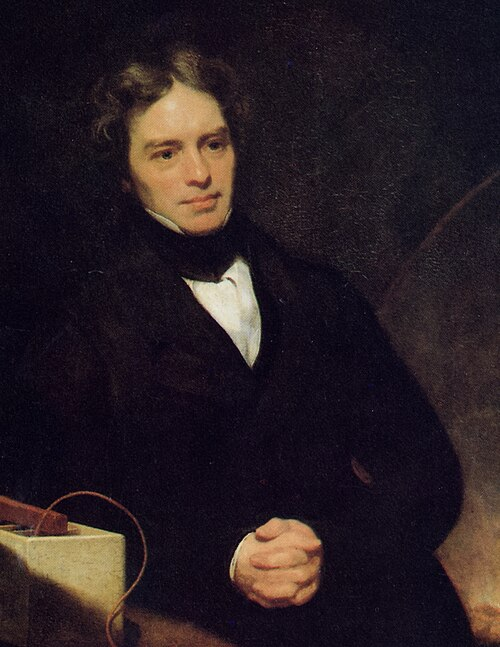
\includegraphics[width=\linewidth]{images/book3/faraday.jpg}
\end{minipage}\hfill
\begin{minipage}[t]{0.69\linewidth}
\vspace{0pt}
في سنة 1834 نص مايكل فاراداي، وهو يقيس نواتج عمليات التحليل الكهربائي
بمقياس فولطي من تصميمه، على أن كتلة المادة الناتجة عند قطب
تتناسب مع كمية الكهرباء المارة، وعلى أن كتل المواد
المختلفة، من أجل كمية معيّنة من الكهرباء، تتناسب مع مكافئاتها الكيميائية.
وهو الذي صاغ كلمات القطب والمصعد والمهبط والأيون والأنيون والكاتيون. والثابت
الذي يحمل اسمه يحوّل هذين القانونين إلى $Q = nF\,\Delta\xi$. (لوحة بريشة توماس فيليبس،
1842، ملكية عامة، ويكيميديا كومنز.)
\end{minipage}
\end{history}

\section{خلايا التركيز}

\begin{definition}[خلية التركيز]\label{def:b2:cell-thermodynamics:concentration-cell}
\emph{خلية التركيز}\index{خلية تركيز} تتكوّن من نصفي
خلية للمزدوجة نفسها لا يختلفان إلا في تركيز (أو
ضغط) نوع كيميائي واحد.
\end{definition}

\begin{proposition}[جهد خلية التركيز]\label{prop:b2:cell-thermodynamics:concentration-cell}
قطبان من فلز M مغموران في محلولين من \ce{M^{n+}} تركيزاهما
$c_1 < c_2$، يصل بينهما جسر ملحي، يعطيان جهدًا
\[
  U = \frac{RT}{nF}\ln\frac{c_2}{c_1} ,
\]
والقطب الموجب هو جهة المحلول الأكثر تركيزًا. وتعمل الخلية حتى يتساوى
التركيزان.
\end{proposition}

\begin{proof}
حسب معادلة نرنست يكون لكل قطب $E_i = E^\circ + (RT/nF)\ln c_i$ (محاليل
مخففة مثالية)؛ ويُختصر $E^\circ$ في الفرق. والتفاعل هو
\babelsublr{\ce{M^{n+}}(\foreignlanguage{arabic}{الجهة 2}) $\to$ \ce{M^{n+}}(\foreignlanguage{arabic}{الجهة 1})}: يترسب الفلز على
الجهة المركزة (المهبط) ويذوب في الجهة المخففة (المصعد)، وهو ما
يسوّي التركيزين؛ و$\Delta_r G = RT\ln(c_1/c_2) < 0$ حتى
يتساويا.
\end{proof}

\begin{omfigure}
\begin{tikzpicture}[font=\small, >={Stealth}]
  \pic at (0,0) {beaker={0.7}{omDef!10}};
  \pic at (3.6,0) {beaker={0.7}{omDef!32}};
  \pic at (-0.3,0.25) {electrode={black!25}};
  \pic at (3.9,0.25) {electrode={black!25}};
  \pic at (0.35,0.55) {saltbridge={2.9}};
  \pic (m) at (1.8,4.3) {meter={V}};
  % common (black) terminal on the anode side, red (+) on the cathode side
  \fill[black] (1.4,4.03) circle (0.065); \fill[red!70!black] (2.2,4.03) circle (0.065);
  \draw[thick] (-0.15,2.65) |- (m-a);
  \draw[thick] (4.05,2.65) |- (m-b);
  \node[anchor=east] at (-0.95,1.0) {\ce{Ag}};
  \node[anchor=west] at (4.45,1.0) {\ce{Ag}};
  \node at (0.25,-0.35) {\babelsublr{\ce{Ag+} \qty{0.010}{mol/L}}};
  \node at (3.6,-0.35) {\babelsublr{\ce{Ag+} \qty{0.10}{mol/L}}};
  \node[anchor=east] at (-0.9,2.3) {\foreignlanguage{arabic}{المصعد $-$}};
  \node[anchor=west] at (4.6,2.3) {\foreignlanguage{arabic}{$+$ المهبط}};
  \node[font=\scriptsize] at (-0.1,-0.8) {\ce{Ag -> Ag+ + e-}};
  \node[font=\scriptsize] at (3.7,-0.8) {\ce{Ag+ + e- -> Ag}};
  \node[font=\scriptsize] at (1.8,5.05) {$U = \qty{59}{mV}$};
\end{tikzpicture}

{\small \omterm{def:b2:cell-thermodynamics:concentration-cell}{خلية تركيز} من الفضة عند \qty{25}{\degreeCelsius}. الجهة المخففة هي
المصعد: تذوب الفضة فيها وتترسب على الجهة المركزة،
حتى يتساوى التركيزان. $U = 0.0592\log(0.10/0.010) =
\qty{59}{mV}$.}
\end{omfigure}

يقيس المبدأ نفسه التراكيز. فقطب الزجاج، الذي يفصل غشاؤه الرقيق
محلولًا مرجعيًا عن العيّنة، ينشأ عليه جهد غشائي قدره
$(RT/F)\ln 10 = \qty{59}{mV}$ لكل وحدة من فرق pH عند
\qty{25}{\degreeCelsius}: فمقياس pH الوارد في مجلد السنة الأولى \omterm{def:b2:cell-thermodynamics:concentration-cell}{خلية تركيز}
لأيونات \ce{H+}. وعبر غشاء الخلية الحية، تُنشئ التراكيز غير المتساوية
لأيونات \ce{K+} بالطريقة نفسها جهدًا من عدة عشرات من الملّيفولطات.

\section{تمارين}

\begin{exercise}[$\star$]\label{exo:b2:cell-thermodynamics:1}
انطلاقًا من $\Delta_f G^\circ(\ce{H2O}, \text{l}) = \qty{-237.14}{kJ/mol}$، احسب
الجهد القياسي لخلية الهيدروجين--الأكسجين.
\end{exercise}

\begin{exercise}[$\star$]\label{exo:b2:cell-thermodynamics:2}
سعة بطارية \qty{1.0}{A.h}. احسب الشحنة التي تختزنها، بالكولوم،
وكتلة الزنك المستهلكة عند مصعدها (\ce{Zn -> Zn^2+ + 2e-}) حين
تُفرَّغ تمامًا.
\end{exercise}

\begin{exercise}[$\star$]\label{exo:b2:cell-thermodynamics:3}
تعطي خلية دانييل \qty{1.10}{V} دون تيار. احسب $\Delta_r G$ لمول واحد
من الزنك والشغل الكهربائي الأقصى لكتلة \qty{10.0}{g} من الزنك.
\end{exercise}

\begin{exercise}[$\star$]\label{exo:b2:cell-thermodynamics:4}
قطبان من النحاس مغموران في محلولين من كبريتات النحاس(II) تركيزاهما \qty{1.0e-3}{mol/L}
و\qty{0.10}{mol/L}. احسب الجهد عند \qty{25}{\degreeCelsius} وسمِّ
القطبين.
\end{exercise}

\begin{exercise}[$\star\star$]\label{exo:b2:cell-thermodynamics:5}
لخلية ($n = 2$) $E^\circ = \qty{1.015}{V}$ و$dE^\circ/dT = \qty{-4.0e-4}{V/K}$
عند \qty{298}{K} (معطيات تمرين). احسب $\Delta_r G^\circ$ و$\Delta_r S^\circ$ 
و$\Delta_r H^\circ$.
\end{exercise}

\begin{exercise}[$\star\star$]\label{exo:b2:cell-thermodynamics:6}
تفرّغ خلية \cref{exo:b2:cell-thermodynamics:5} مولًا واحدًا من التفاعل
(أ) عكوسيًا؛ (ب) عند \qty{0.90}{V}. احسب في كل حالة الشغل الكهربائي 
والحرارة المتبادلة مع الوسط المحيط.
\end{exercise}

\begin{exercise}[$\star\star$]\label{exo:b2:cell-thermodynamics:7}
احسب $E^\circ(\ce{Fe^3+}/\ce{Fe})$ من طاقات جيبس للتكوين
(\ce{Fe^2+} \qty{-78.90}{kJ/mol}، \ce{Fe^3+} \qty{-4.7}{kJ/mol}) وتحقق من أنه
يساوي $(E_1^\circ + 2E_2^\circ)/3$.
\end{exercise}

\begin{exercise}[$\star\star$]\label{exo:b2:cell-thermodynamics:8}
احسب الجهد المعياري للمزدوجة $\ce{AgCl}/\ce{Ag}$، ثم
جهد قطب كلوريد الفضة المغمور في محلول كلوريد البوتاسيوم بتركيز \qty{0.10}{mol/L}.
\end{exercise}

\begin{exercise}[$\star\star$]\label{exo:b2:cell-thermodynamics:9}
تستعمل خلايا الزنك--الهواء التفاعل \ce{2Zn + O2 -> 2ZnO} ($\Delta_f G^\circ(\ce{ZnO}) =
\qty{-318.30}{kJ/mol}$). احسب الجهد القياسي والطاقة الكهربائية
القصوى، بوحدة \unit{kW.h}، لكل كيلوغرام من الزنك.
\end{exercise}

\begin{exercise}[$\star\star\star$]\label{exo:b2:cell-thermodynamics:10}
تشغّل خلية وقود الميثانول المباشرة التفاعل \ce{CH3OH(l) + 3/2O2 -> CO2 + 2H2O(l)}. انطلاقًا من
$\Delta_f H^\circ$ (\unit{kJ/mol}): \ce{CH3OH(l)} $-239$، \ce{CO2} $-393.51$،
\ce{H2O(l)} $-285.83$؛ ومن $S^\circ$ (\unit{J/(K.mol)}): \ce{CH3OH(l)} 127.2،
\ce{CO2} 213.8، \ce{H2O(l)} 69.95، \ce{O2} 205.15، احسب $n$ و$E^\circ$ 
والمردود الأقصى.
\end{exercise}

\begin{exercise}[$\star\star\star$]\label{exo:b2:cell-thermodynamics:11}
لخلية ($n = 2$) $E = \qty{0.500}{V}$ و$dE/dT = \qty{+3.0e-4}{V/K}$ عند
\qty{298}{K} (معطيات تمرين). بيّن أنها، إذ تعمل عكوسيًا، تعطي شغلًا
كهربائيًا أكبر من $-\Delta_r H$، وفسّر من أين تأتي الطاقة الزائدة.
\end{exercise}

\begin{exercise}[$\star\star\star$]\label{exo:b2:cell-thermodynamics:12}
قطبا هيدروجين (\qty{1}{bar} من \ce{H2}) مغموران في محلول مرجعي
قيمة pH له 7.00 وفي عيّنة. الجهد \qty{0.177}{V} عند \qty{25}{\degreeCelsius}،
والمرجع هو القطب الموجب. أوجد قيمة pH للعيّنة، وفسّر
لماذا لا تتعلق النتيجة بأي جهد معياري.
\end{exercise}

\section{مسألة: حافلة خلايا الوقود}

\begin{problem}[{مسألة نهاية الأسبوع --- الجهد القياسي لخلية
الهيدروجين--الأكسجين من طاقات جيبس، ومعاملها الحراري، ومردود
مكدس حقيقي وحرارته، والطاقة في خزان من الهيدروجين}]
\label{pb:b2:cell-thermodynamics:1}
مكدس خلايا وقود فيه 400 خلية على التوالي، لكل منها غشاء
تبادل بروتوني (إلكتروليت حمضي). المعطيات عند \qty{298.15}{K} (كوداتا، جاناف):
$\Delta_f H^\circ(\ce{H2O}, \text{l}) = \qty{-285.83}{kJ/mol}$، $\Delta_f
G^\circ(\ce{H2O}, \text{l}) = \qty{-237.14}{kJ/mol}$، $\Delta_f G^\circ(\ce{H2O},
\text{g}) = \qty{-228.58}{kJ/mol}$؛ $S^\circ$ (\unit{J/(K.mol)}): \ce{H2O(l)} 69.95،
\ce{H2} 130.68، \ce{O2} 205.15. $F = \qty{96485}{C/mol}$؛ $M(\ce{H2}) =
\qty{2.016}{g/mol}$.
% ledger: dfh:H2O-l, janafG:H2O_l.298, janafG:H2O.298, s0:H2O_l, s0:H2_g, s0:O2_g, const:F, aw:H

\medskip
\noindent\textbf{الجزء الأول --- الجهد القياسي.}
\begin{enumerate}
  \item اكتب نصفي التفاعل عند المصعد وعند المهبط، وتفاعل
        الخلية.
  \item كم إلكترونًا يُتبادل لكل جزيء من الهيدروجين؟
  \item احسب $E^\circ$ حين يتكوّن الماء سائلًا.
  \item احسبه حين يغادر الماء بخارًا.
  \item فسّر الفرق \omterm{def:b2:reaction-free-energy:gibbs-energy}{بطاقة جيبس} لتبخر الماء.
  \item احسب $\Delta_r H^\circ$ والمردود الأقصى عند \qty{298}{K}.
\end{enumerate}

\medskip
\noindent\textbf{الجزء الثاني --- درجة الحرارة.}
\begin{enumerate}[resume]
  \item احسب $\Delta_r S^\circ$ من أجل الماء السائل.
  \item استنتج $dE^\circ/dT$.
  \item قدّر $E^\circ$ عند \qty{80}{\degreeCelsius}، وهي درجة حرارة تشغيل
        المكدس.
  \item قارن طريقتك بقيمة جاناف عند \qty{400}{K}، $\Delta_f
        G^\circ(\ce{H2O}, \text{l}) = \qty{-221.01}{kJ/mol}$.
  \item ما الحرارة التي تتبادلها الخلية العكوسة لكل مول من الهيدروجين عند
        \qty{298}{K}؟ وهل هي مستقبَلة أم محررة؟
  \item قدّر المردود الأقصى عند \qty{80}{\degreeCelsius}.
\end{enumerate}

\medskip
\noindent\textbf{الجزء الثالث --- المكدس الحقيقي عند \qty{0.70}{V} لكل خلية.}
\begin{enumerate}[resume]
  \item احسب الشغل الكهربائي لكل مول من الهيدروجين.
  \item احسب المردود منسوبًا إلى $\Delta_r H^\circ$ وإلى $\Delta_r G^\circ$.
  \item احسب الحرارة المحررة لكل مول من الهيدروجين.
  \item كم منها لا مفر منه، وكم يعود سببه إلى التيار؟
  \item يعطي المكدس \qty{300}{A}. احسب استهلاك الهيدروجين لخلية
        واحدة، ثم للمكدس، بالمولات وبالغرامات في الثانية.
  \item احسب الاستطاعة الكهربائية للمكدس.
  \item احسب الاستطاعة الحرارية التي يجب أن تصرفها دارة التبريد.
\end{enumerate}

\medskip
\noindent\textbf{الجزء الرابع --- الخزان.}
\begin{enumerate}[resume]
  \item ما كمية مادة الهيدروجين في \qty{5.0}{kg}؟
  \item ما الشحنة التي تمر عبر الخلايا، محسوبة على مجموعها كلها، حين
        يتأكسد هذا الهيدروجين؟
  \item احسب الطاقة الكهربائية التي يعطيها المكدس، وكل خلية عند
        \qty{0.70}{V}.
  \item حوّلها إلى كيلوواط ساعي.
  \item ما المدة التي يستطيع المكدس خلالها إعطاء استطاعته المحسوبة في السؤال 18؟
  \item اذكر الطاقة الكهربائية التي تعطيها \qty{5.0}{kg} من الهيدروجين عند
        \qty{0.70}{V} لكل خلية.
\end{enumerate}
\end{problem}
